
In the last experiment we calibrated the \pipulse and, having already calibrated the measurement pulse, we have all the components needed for control, technically we could already perform algorithmic experiments.
However, we still do not know much about the qubit itself and, in particular, the values of $T_1$ and $T_2$.
Moreover, we didn't perform a complete calibration and, if we tried to run circuits now, we will not achieve good fidelities.

The \textit{Ramsey experiment}~\cite{Ramsey1950} is a simple routine that allows us to address all these problem at once. 
In particular, with it we can:
\begin{itemize}
    \item fine tune the drive qubit frequency;
    \item perform a sanity check on our setup, confirming we are correctly controlling signals phases;
    \item compute $T_2$ (technically we obtain $T_2^\star$, see footnote)
\end{itemize}

The experiment can be performed in a \textit{simpler} version, often called \textit{non-detuned Ramsey} and in a \textit{detuned} version.

Although usually the non-detuned experiment can be avoided, it is useful as a starting point for the discussion.
So, let's start from it. 

First, we send to the drive line a \pihpulse.
That is a drive pulse with the same characteristics of a \pipulse, but with the amplitude halved.
This pulse should work as follows:
\begin{align*}
    \ket 0 &\xrightarrow{\frac{\pi}{2}} \frac{\ket 0 + i\ket 1}{2}\\
    \ket 1 &\xrightarrow{\frac{\pi}{2}} \frac{\ket 0 - i\ket 1}{2} 
\end{align*}

After the \pihpulse, we wait for a certain time and fire a second \pihpulse followed by a measurement.
We then repeat the experiment for increasing waiting times between pulses and we plot the measured amplitude against the waiting times.
\textit{In the ideal case}, we expect to see an exponential decay from the amplitude corresponding to $\ket 1$ to the medium point between ground and excited state.
At this point we can fit the obtained curve with an exponential and obtain $T_2$ as the decaying constant\footnote{Technically we obtain $T_2^\star$ in this experiment. See \cref{sec:t2_spin_echo} for more details.}.

It is not immediate to understand what is happening to the qubit, but we can try starting at the limit values:
\begin{itemize}
    \item at wait time $0$, we send two consecutive \pihpulse that have, together, the same effect of a \pipulse, so we expect to measure the excited state;
    \item at wait time $\gg T_2$, we expect the qubit to decohere during the waiting time (we are not considering relaxation since in general $T_1\gg T_2$). So we expect to be again in complete superposition when we measure;
\end{itemize}

but what happens for an intermediate waiting time?\\
After the first pulse, the qubit start to decohere so a variable phase gets added to the state.
We can visualize this decoherence as a rotation on the xy plane, in the Bloch sphere.
When we apply the second pulse, we have an equal probability to get to the ground state or to the excited one since the phase added is not constant.

We can see a schematic representation of the experiment in \cref{fig:ramsey_experiment}.
\begin{figure}[ht]
    \centering
    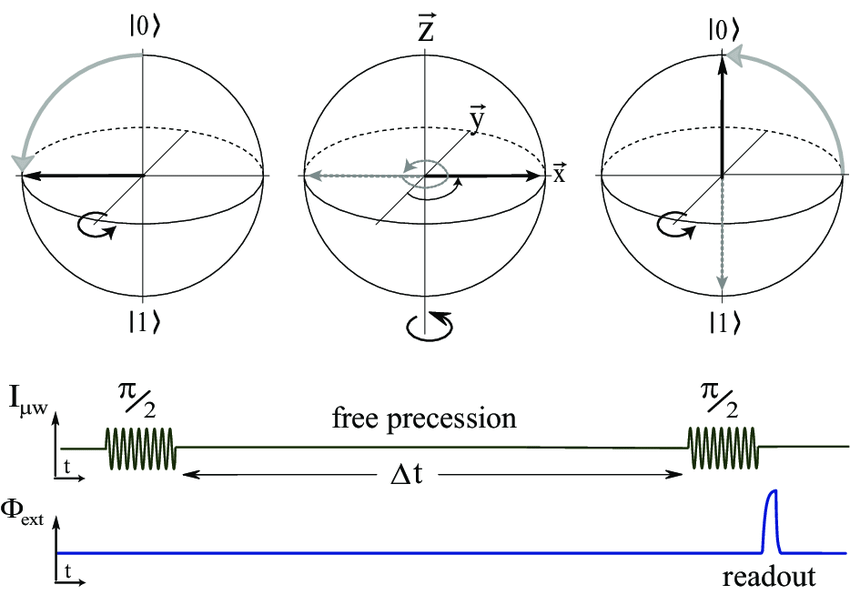
\includegraphics[width=0.8\textwidth]{characterization/figures/ramsey_experiment.png}
    \caption{Schematic representation of a Ramsey experiment. Credits~\cite{ramsey_experiment}.}
    \label{fig:ramsey_experiment}
\end{figure}

The ideal plot is presented in the sketch in \cref{fig:ideal_ramsey_sketch}

\begin{figure}[ht]
    \centering
    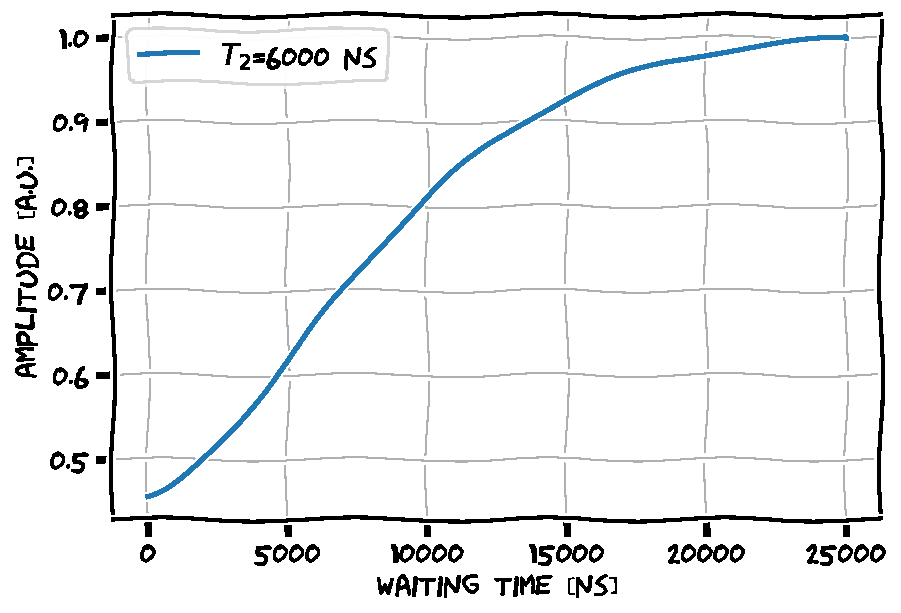
\includegraphics[width=8cm]{characterization/figures/ramsey_sketch.pdf}
    \caption{Sketch of the plot of a Ramsey experiment in ideal conditions.}
    \label{fig:ideal_ramsey_sketch}
\end{figure}

However, several effects could lead to spurious and unexpected behaviours.
Consider for example \cref{fig:spurious_coupling_ramsey}.
A part from some noise that has to be expected, here the plot is almost ideal and the curve, obtained by points average 1000 times, can be easily fitted with an exponential (a $T_2=6\,\mu$s was extracted). 
But what happens around $13$ thousands ns and again around $17$ and $20$ is not just noise: indeed we can see that the qubit state is "constantly" having a different final state. This can happen when the qubit, because of a non perfect environmental isolation, couples to spurious cavity modes, thus effectively changing the 0-1 transition frequency.

\begin{figure}[ht]
    \makebox[\textwidth][c]{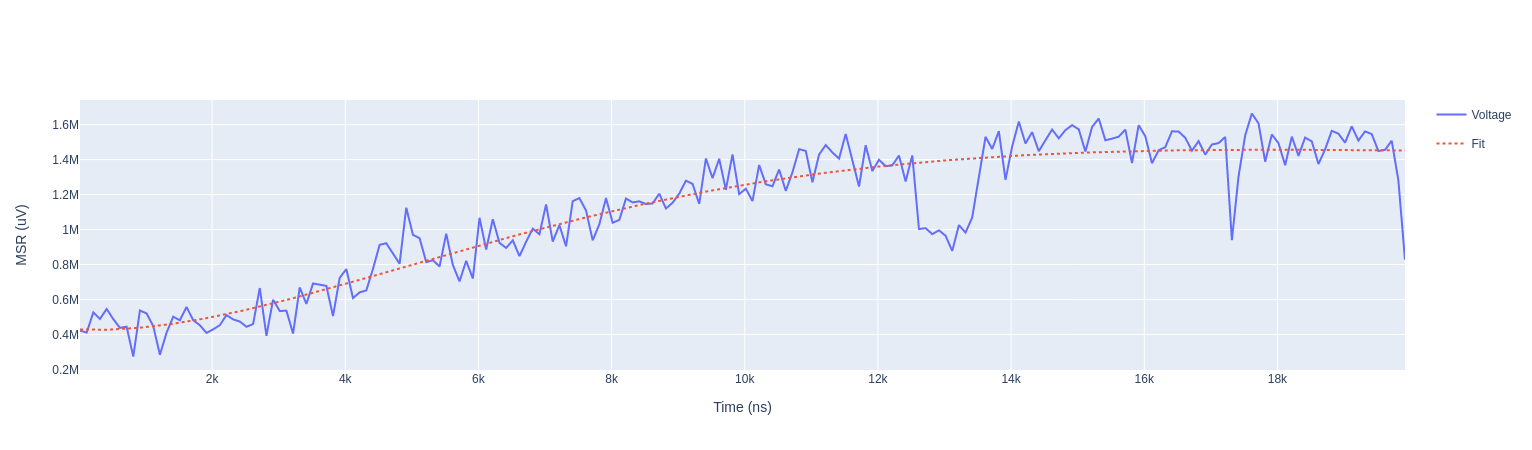
\includegraphics[width=1.3\textwidth]{characterization/figures/ramsey_spurious_coupling.png}}
    \caption{Plot for a Ramsey experiment with the presence of a spurious coupling.}
    \label{fig:spurious_coupling_ramsey}
\end{figure}

Another possible plot that one could obtain is presented in \cref{fig:ramsey_experiment_wrong_freq}.
\begin{figure}[ht]
    \makebox[\textwidth][c]{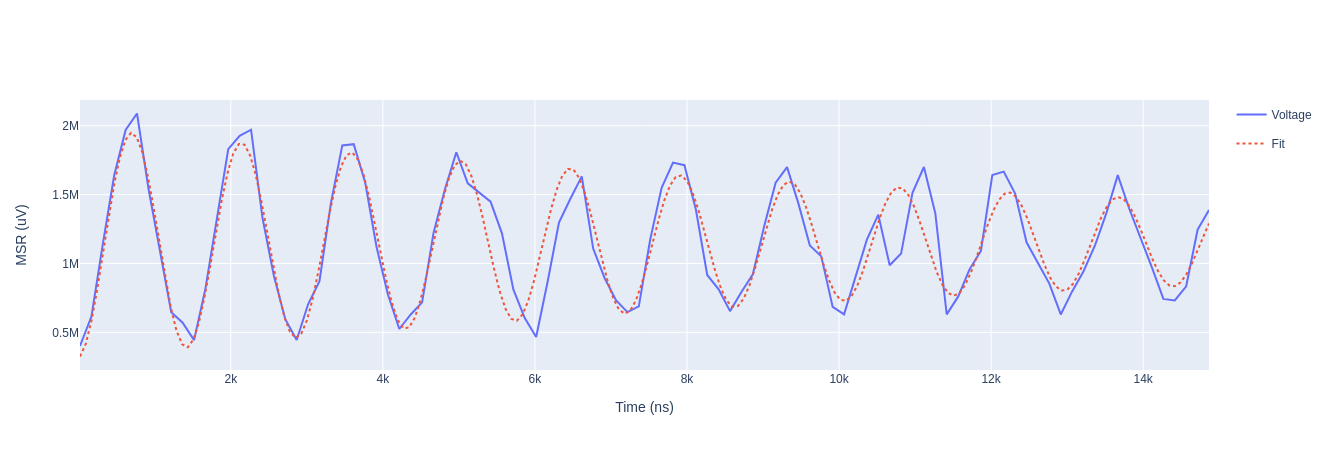
\includegraphics[width=1.3\textwidth]{characterization/figures/ramsey_wrong_freq.png}}
    \caption{Plot for a Ramsey experiment at the wrong drive frequency.}
    \label{fig:ramsey_experiment_wrong_freq}
\end{figure}
Actually, the majority of the times, when we perform a Ramsey experiment we will initially obtain something like this. 
Note that we still have the exponential decay but convoluted with a sinusoidal.
This can be explained with a not-properly-calibrated \pipulse (and therefore a not-properly-calibrated \pihpulse).
Indeed if our drive pulse is not sending $\ket 0$ into $\frac{\ket 0 + i\ket 1}{2}$, but in something near it \textit{outside} the xy plane, than the decohering will happen as a rotation also outside the xy plane.
So, for example, when we have wait time equal to zero, then we are not doing exactly a rotation over x of $\pi$, but of $\pi\pm\epsilon$ where $\epsilon$ is usually small.\\
Therefore we are seeing the decoherence of Ramsey and the oscillations of Rabi at the same time.

From the period of the oscillations we can fine tune the drive frequency.
In the plot of \cref{fig:ramsey_experiment_wrong_freq}, for example, the oscillations have a period of $\approx 1.8\,\mu$s, this means that the frequency is off by $\frac{1}{1.8\,\mu\text{s}}=555555$ Hz.
Basically, we are performing a fit with:
\begin{equation}\label{eq:ramsey_fit}
    y = p_0 + p_1\sin\left( 2\pi\Delta x + p_3 \right) e^{-\frac{x}{T_2}} 
\end{equation}
with the final correction being $\Delta$.

The problem, at this point, is knowing the sign of the correction to which we are currently not sensible at all.
We have the option of trying the two values and choose the one that produces the most exponential-like curve.
Note, also, that for every change in the frequency, it is recommended to perform a new Rabi experiment to re-calibrate the \pipulse.

The other option, to avoid the sign ambiguity, is to perform the detuned experiment.\\
We start defining the maximum wait time we will probe as $max\_wait$ and a number of desired oscillations as $n$.
For every second \pihpulse, we will add a spurious phase defined as:
\begin{equation}
    \phi = (\text{start\_time})2\pi \frac{n}{max\_wait}
\end{equation}
The effect of this detuning, if the drive frequency is the exact one will present itself as precisely $n$ oscillations in the plots.
On the other hand, if we are driving the qubit at a higher frequency we expect to see more oscillations, if we are not driving the qubit enough we will see less.
The fit function is again \cref{eq:ramsey_fit}, but the final correction become:
\begin{equation}
    \Delta_{corr} = \Delta - \frac{n}{max\_wait}
\end{equation}
with the new drive frequency being $\omega_q = \omega_d - \Delta_{corr}$\footnote{A wrong interpretation of the phase, that here is defined as positively growing with growing frequencies, will lead to $\omega_q = \omega_d + \Delta_{corr}$.}.

After the correction and after a new \textit{required} Rabi experiment, is always advisable to repeat the non-detuned experiment, to really check if the oscillation is disappeared (so to check if the drive frequency is now correct).

\experimentrecap
{Ramsey experiment}
{drive calibration, qubit characterization}
{fine tuned qubit/drive frequency,\\characteristic dephasing time $T_2$ ($T_2^\star$)}
{a \pihpulse is sent to the qubit through the drive line, after a variable wait time we execute a new \pihpulse and measure.
If we do not see any oscillation, but just an exponential decay, we can find $T_2$. Otherwise, depending on the number of oscillations we can fine tune the drive frequency with a sign ambiguity, perform a Rabi experiment e repeat the Ramsey experiment. In the detuned version of the experiment, a spurious and controlled detuning is introduced as a phase on the second \pihpulse. The effect is to fix a desired number of oscillations as $\neq 0$ and, if this number is different from what expected, we can again fine tune the frequency without sign ambiguity}

